\chapter{Teoria cinetica dei gas}
\section{Ipotesi}
La teoria cinetica dei gas si basa sulle seguenti ipotesi:
\begin{itemize}
	\item Elevata densit� molecolare
	\item	Elevata distanza intermolecolare rispetto le dimensioni delle molecole
	\item	Molecole non interagenti tra di loro
	\item	Distribuzione molecolare uniforme
	\item	Tutte le direzioni di moto equalmente probabili
\end{itemize}

\section{Energia cinetica del gas}
Consideriamo una superficie A contro cu avvengono gli urti delle molecole di gas, come raffigurato in \figurename~\ref{fig:TCG:UrtoParete}.
\begin{figure}[htbp]
	\centering
		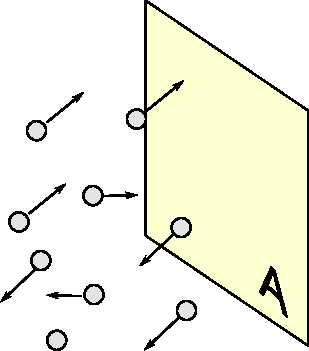
\includegraphics[width=0.40\textwidth]{image/TCGUrtoParete.pdf}
	\caption{Rappresenzatione schematica del meccanismo di base su cui si basa la Teoria Cinetica del Gas}
	\label{fig:TCG:UrtoParete}
\end{figure}
si possono determinare, per ogni particella, la distanza della parte:
\begin{equation}
	x = v_x \cdot \Delta t
	\label{eq:DistanzaParteParticella}
\end{equation}
e il numero di urti che subisce la partete:
\begin{equation}
	n_{urti} = \frac{1}{2} v_x \cdot \Delta t \cdot A \cdot N
	\label{eq:NumeroUrtiParete}
\end{equation}
dove $N$ � la densit� di molecole ($\frac{n}{V}$), mentre il fattore moltiplcativo $\frac{1}{2}$ � dovuto al fatto che le molecole si muovono nelle due direazioni di ogni asse, quindi solo la met� di esse avr� direzione utile per colpire la parte A.

La variazione di quantit� di moto a seguito di un urto � pari a:
\begin{equation}
	\Delta q = q_1 - q_2 = m \cdot v_x - (-v_x \cdot m) = 2 m \cdot v_x
	\label{eq:VariazQuantitaMoto1}
\end{equation}
dove la velocit� a seguito dell'urto ha direzione inversa, mentre, essendo l'urto elastico, ha lo stesso modulo.

La variazione della quantit� di moto totale sar� pari a:
\begin{equation}
	\Delta q_{TOT} = (\frac{1}{2} v_x \cdot \Delta t \cdot A \cdot N) \cdot (2 m \cdot v_x)
								 = m \cdot v_x^2 \cdot \Delta t \cdot A \cdot N
	\label{eq:VariazQuantitaMotoTot}
\end{equation}
che riarrangiata porta a 
\begin{equation}
	\frac{\Delta q_{TOT}}{A \cdot \Delta t} = m \cdot v_x^2 \cdot N
	\label{eq:VariazQuantitaMotoTotRiarr}
\end{equation}
Essendo $q = m \cdot v$, $a = \frac{v}{\Delta t}$, $F = m 	\cdot a$ e anche $P = \frac{F}{A}$ otteniamo:
\begin{equation}
	\frac{\Delta q_{TOT}}{A \cdot \Delta t} = \frac{F}{A} = P = m \cdot v_x^2 \cdot \frac{n}{V}
	\label{eq:Pressione}
\end{equation}
da cui ricaviamo anche:
\begin{equation}
	\frac{P V}{n} = m \cdot v_x^2
	\label{eq:EnergCientica1}
\end{equation}

Essendo per le ipotesi iniziali tutte le direzioni di moto egualmente probabili, si ha:
\begin{equation}
	<v>^2 = <v_x>^2 + <v_y>^2 + <v_z>^2 = 3 \cdot <v_x>^2
	\label{eq:Velocita2}
\end{equation}
quindi
\begin{equation}
	\frac{P V}{n} = R T =  m \cdot v_x^2 = m \cdot (\frac{1}{3} <v>^2)
	\label{eq:EnergCientica2}
\end{equation}
da cui si ricava il valore dell'energia cinetica media di un gas, che risulta essere paria a: 
\begin{equation}
	\frac{1}{2} m <v>^2 = \frac{3}{2} R \cdot T
	\label{eq:EnergCientica}
\end{equation}

%==============================================================================================
\section{Frequenza d'urto tra due particelle}
Determianiamo ora la frequenza d'urto tra due particelle gassose, ipotizzando che abbiano una struttura sferica, come rappresentato in \figurename~\ref{fig:TCG:UrtoParticelle}.
\begin{figure}[htbp]
	\centering
		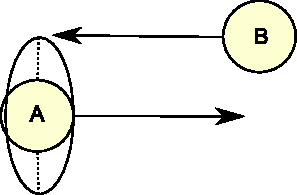
\includegraphics[width=0.40\textwidth]{image/TCGUrtoParticelle.pdf}
	\caption{Rappresenzatione schematica di un urto tra due particelle gassose.}
	\label{fig:TCG:UrtoParticelle}
\end{figure}

Il numero di urti di una particella � dato da 
\begin{equation}
	n_{urti} = \pi \cdot D^2 \cdot <v> \cdot \Delta t \cdot N
	\label{eq:UrtiParticella}
\end{equation}
mentre la frequenza di urti totali � data da:
\begin{equation}
	\frac{n_{urti TOT}}{\Delta t} = (\pi \cdot D^2 \cdot <v> \cdot N) \cdot N
	\label{eq:FreqUrtiParticella}
\end{equation}

Poich� se la particella A urta la particella B anche B urta A bisogna moltiplicare questo valore per $\frac{1}{2}$ per ottenere il numero reale di urti, inoltre poich� le particelle si muovono bisogna moltiplicare per un fattore statistico pari a $\sqrt{2}$, quindi abbiamo:
\begin{equation}
	z = \frac{\sqrt{2}}{2} \pi D^2 \cdot <v> \cdot N^2
	\label{eq:FreqUrtiParticellaZ}
\end{equation}

Se ogni urto tra due molecole � reattivo $z$ � anche la velocit� di reazione, quindi per la generica reazione 
\begin{equation}
	A\cdot + A\cdot \rightarrow A_2
	\label{eq:Reazione}
\end{equation}
e la relativa velocit� di reazione sar�:
\begin{equation}
	r = z = \frac{\sqrt{2}}{2} \pi D^2 \cdot <v> \cdot N^2 = k_{RXN} \cdot C_A^2
	\label{eq:VelocitaReazione}
\end{equation}
da cui si evince che la costante cinetica �:
\begin{equation}
	k_{RXN} = \frac{\sqrt{2}}{2} \pi D^2 \cdot <v>
	\label{eq:CostCinetica}
\end{equation}

%==============================================================================================
\section{Distribuzione della velocit� secondo Boltzman}
Affrontiamo ora la distribuzione delle velocit� molecolari come � stato fatto da Boltzman\footnote{Boltzmann, Ludwig (Vienna 1844 - Duino 1906), fisico austriaco.} nel 1869.

Indichiamo con $f_{(v)}$ la funzione di distribuzione delle velocit�, possiamo scomporla rispetto ai tre assi cartesiani, avendo cos�:
\begin{equation}
	f_{(v)} = f_{(v_x)} + f_{(v_y)} + f_{(v_z)}
	\label{eq:VelocitaScomposta}
\end{equation}

Le molecole con velocti� $\vec{v}$ compresa tra $v_x$ e $v_x + dv_x$ saranno:
\begin{equation}
	\frac{dN_{v_x}}{N} = f_{(v_x)} d v_x
	\label{eq:dNx}
\end{equation}
mentre le velocit� medie diventeranno:
\begin{equation}
	<v_x> = \frac{\int v_x dN_{v_x}}{\int dN_{v_x}} = 
					\frac{\int v_x f_{(v_x)} d v_x}{\int f_{(v_x)} d v_x} = 
	\label{eq:VelocitaMedia}
\end{equation}
essendo la velocit� data da:
\begin{equation}
	\vec{v} = \vec{i} \cdot v_x + \vec{j} \cdot v_y + \vec{k} \cdot v_z
	\label{eq:ComposizioneVelocita}
\end{equation}

consideriamo una corona sferica di spessore $d v$ e l'ipotesi di Maxwell\footnote{Maxwell, James Clerk (Edimburgo 1831 - Cambridge 1879), fisico britannico} applicata alla distribuzione di una popolazione si ha:
\begin{equation}
	d N_{v_x} \cdot d N_{v_y} \cdot d N_{v_z} = N \cdot f_{(v_x)} d v_x \cdot 
																								f_{(v_y)} d v_y \cdot 
																								f_{(v_z)} d v_z
	\label{eq:dN}
\end{equation}
e quindi 																								
\begin{equation}
	d^3 N_{v_x, v_y, v_z} = N \cdot f_{(v_x)} \cdot f_{(v_y)} \cdot f_{(v_z)} d v_x d v_y  d v_z
	\label{eq:d3N}
\end{equation}
e ancora:
\begin{equation}
	\frac{d^3 N_{v_x, v_y, v_z}}{d v_x d v_y  d v_z} = 	N \cdot f_{(v_x)} \cdot f_{(v_y)} \cdot f_{(v_z)} =
			\sigma_{(v_x, v_y, v_z)}
	\label{eq:d3N_RispettoXYZ}
\end{equation}

Poich� la $v$ � isotropa e la densit� $\sigma$ non � funzione di $\vec{v}$ ma � costante, abbiamo:
\begin{equation}
	d \sigma = 0 = N \cdot (f_{(v_x)}' \cdot f_{(v_y)} \cdot f_{(v_z)})d v_x +
								 N \cdot (f_{(v_x)} \cdot f_{(v_y)}' \cdot f_{(v_z)})d v_y +
								 N \cdot (f_{(v_x)} \cdot f_{(v_y)} \cdot f_{(v_z)}')d v_z
	\label{eq:dDensitaNullo}
\end{equation}
\begin{equation}
	d v = 0 =	v_x d v_x +	v_y d v_y +	v_z d v_z
	\label{eq:dVelocitaNullo}
\end{equation}
Dividendo tutti i membri dell'equazione \ref{eq:dDensitaNullo} per $(f_{(v_x)} \cdot f_{(v_y)} \cdot f_{(v_z)})$ e semplificando $N$ otteniamo:
\begin{multline}
	\frac {f_{(v_x)}' \cdot f_{(v_y)} \cdot f_{(v_z)}}
				{f_{(v_x)} \cdot f_{(v_y)} \cdot f_{(v_z)}} d v_x+ 
	\frac {f_{(v_x)} \cdot f_{(v_y)}' \cdot f_{(v_z)}}
				{f_{(v_x)} \cdot f_{(v_y)} \cdot f_{(v_z)}} d v_y +
	\frac {f_{(v_x)} \cdot f_{(v_y)} \cdot f_{(v_z)}'}
				{f_{(v_x)} \cdot f_{(v_y)} \cdot f_{(v_z)}}	d v_z = \\
	\frac {f_{(v_x)}'}{f_{(v_x)}} d v_x + 
	\frac {f_{(v_y)}'}{f_{(v_y)}} d v_y + 
	\frac {f_{(v_z)}'}{f_{(v_z)}} d v_z =	0
	\label{eq:dDensitaNulloDivisoFvXYZ}
\end{multline}
essendo:
\begin{align}
		f_{(v_x)}' & = \frac{\partial f_{(v_x)}}{\partial v_x} &
		f_{(v_y)}' & = \frac{\partial f_{(v_y)}}{\partial v_y} &
		f_{(v_z)}' & = \frac{\partial f_{(v_z)}}{\partial v_z} 
	\label{eq:DefinizioniDFv}
\end{align}
abbiamo:
\begin{equation}
	\frac {1}{f_{(v_x)}} \frac{\partial f_{(v_x)}}{\partial v_x} d v_x + 
	\frac {1}{f_{(v_y)}} \frac{\partial f_{(v_y)}}{\partial v_y} d v_y + 
	\frac {1}{f_{(v_z)}} \frac{\partial f_{(v_z)}}{\partial v_z} d v_z =	0
	\label{eq:dDensitaNulloDivisoFvXYZ_sostituitoDerivate}
\end{equation}

Per risolvere l'equazione cos� ottenuta si utilizza il metodo dei moltiplicatori indeterminati di Lagrange\footnote{Lagrange, Giuseppe Luigi (Torino 1736 - Parigi 1813), matematico e astronomo italiano di origine francese.}.
Moltiplichiamo le equazione \ref{eq:dVelocitaNullo} per $\lambda$ 
\begin{equation}
	d v = 0 =	v_x \cdot \lambda d v_x +	v_y \cdot \lambda d v_y +	v_z \cdot \lambda d v_z
	\label{eq:dVelocitaNulloLambda}
\end{equation}
sommiamola l'equazione appena ottenuta alla \ref{eq:dDensitaNulloDivisoFvXYZ_sostituitoDerivate} ricavando, cos�:
\begin{multline}
	\left(\frac {1}{f_{(v_x)}} \frac{\partial f_{(v_x)}}{\partial v_x} + v_x \cdot \lambda \right) d v_x + 
	\left(\frac {1}{f_{(v_y)}} \frac{\partial f_{(v_y)}}{\partial v_y} + v_y \cdot \lambda \right) d v_y + \\
	\left(\frac {1}{f_{(v_z)}} \frac{\partial f_{(v_z)}}{\partial v_z} + v_z \cdot \lambda \right) d v_z = 0
	\label{eq:dDensitaNulloDivisoFvXYZ_sostituitoDerivate}
\end{multline}
L'equazione cos� ottenuta risulta soddisfatta se tutti i tre membri nelle parentesi risultano nulli:
\begin{multline}
	\frac {1}{f_{(v_x)}} \frac{\partial f_{(v_x)}}{\partial v_x} + v_x \cdot \lambda = 0\\
	\frac {1}{f_{(v_x)}} \frac{\partial f_{(v_x)}}{\partial v_x} = - v_x \cdot \lambda \\
	\frac {1}{f_{(v_x)}}d f_{(v_x)} = - v_x \cdot d v_x \lambda \\
	ln \left(f_{(v_x)}\right) = - \frac{\lambda}{2} \cdot v_x^2 + C\\
	f_{(v_x)} = e^{- \frac{\lambda}{2} \cdot v_x^2 + C} = \alpha \cdot e^{- \frac{\lambda}{2} \cdot v_x^2}
	\label{eq:SoluzEquazMoltiplicLagrange}
\end{multline}
Bisogna ora determinare le due costanti $\alpha$ e $\lambda$; ricordando l'equazione \ref{eq:dNx}, integrata risulta:
\begin{equation}
	\int_{-\infty}^\infty dN_{v_x} = \int_{-\infty}^\infty  f_{(v_x)} d v_x = \int_{-\infty}^\infty \alpha \cdot e^{- \frac{\lambda}{2} \cdot v_x^2} dv_x
	\label{eq:dNxIntegrata}
\end{equation}
la cui soluzione porta a determinare $\alpha=\sqrt{\frac{\lambda}{\pi}}$

Come seconda condizione al contorno si ricorda l'equazione dell'energia cinetica di un gas (equazione \ref{eq:EnergCientica}) dove la $<v_x^2>$ deriva dall'equazione \ref{eq:VelocitaMedia}:
\begin{equation}
	<v_x^2> = \frac	{\int_0^\infty v_x^2 f_{(v_x)} d v_x}
									{\int_0^\infty f_{(v_x)} d v_x} =
						\frac	{\frac{1}{4}\sqrt{\frac{\pi 2^3}{\lambda^3}}}
									{\frac{1}{2}\sqrt{\frac{\pi 2}{\lambda}}} = \frac{1}{\lambda}
	\label{eq:VelocitaMediaIntegrata}
\end{equation}
Poich� la velocit� media quadratica � pari a:
\begin{equation}
	<v^2> = <v_x^2> + <v_y^2> + <v_z^2> 
				= \frac{1}{\lambda} + \frac{1}{\lambda} + \frac{1}{\lambda} 
				= \frac{3}{\lambda}
	\label{eq:ValoreVRispettoLambda}
\end{equation}
Considerando un'unica molecola, per l'equazione \ref{eq:EnergCientica} abbiamo:
\begin{equation}
	<v^2> = \frac{3 \cdot K_B \cdot T}{m}
	\label{eq:EnergiaCineticaParticella}
\end{equation}
che inserita nell'equazione \ref{eq:ValoreVRispettoLambda} ci porta a ricavare $\lambda$
\begin{equation}
	\frac{3}{\lambda} = <v^2> = \frac{3 \cdot K_B \cdot T}{m} \Rightarrow \lambda = \frac{m}{K_B \cdot T}
	\label{eq:Lambda}
\end{equation}
che ci permette di determinare $\alpha$:
\begin{equation}
	\alpha = \sqrt{\frac{\lambda}{\pi}} = \sqrt{ \frac{m}{K_B \cdot T} \frac{1}{\pi}}
	\label{eq:alfa}
\end{equation}

Tornando alla funzione di distribuzione delle velocit� abbiamo:
\begin{equation}
	f_{(v_x)} = \alpha \cdot e^{- \frac{\lambda}{2} \cdot v_x^2} = \sqrt{ \frac{m}{K_B \cdot T} \frac{1}{\pi}} \cdot e^{- \frac{m}{2 K_B \cdot T} \cdot v_x^2}
	\label{eq:FunzDistribVxRisolta}
\end{equation}
e, considerando le tre dimensioni:
\begin{multline}
	f_{(v_x, v_y, v_z)} = f_{(v_x)} \cdot f_{(v_y)} \cdot f_{(v_z)} =\\
											 \left(\frac{m}{\pi \cdot K_B \cdot T}\right)^\frac{3}{2} \cdot 
											 e^{- \frac{m}{2 K_B \cdot T} \cdot \left(v_x^2 + v_y^2 + v_z^2\right)} = \\
											 \left(\frac{m}{\pi \cdot K_B \cdot T}\right)^\frac{3}{2} \cdot 
											 e^{- \frac{m}{2 K_B \cdot T} \cdot v^2}
	\label{eq:FunzDistribVxyzRisolta}
\end{multline}

Essendo per definizione
\begin{equation}
	<v> = \frac{\int_0^\infty v dN_{v}}{\int_0^\infty dN_{v}} = 
					\frac{\int_0^\infty v f_{(v)} d v}{\int_0^\infty f_{(v)} d v} =
					\sqrt{\frac{8 \cdot K_B \cdot T}{\pi \cdot m}}
	\label{eq:VelocitaMediaIntegrata2}
\end{equation}
Per quanto visto precedentemente (equazione \ref{eq:FreqUrtiParticella}) la frequenza d'urto tra due particelle uguali risulter�
\begin{equation}
	z_{A-A} = \frac{\sqrt{2}}{2} \pi D_A^2 \cdot <v> \cdot N^2 =
						\frac{\sqrt{2}}{2} \pi D_A^2 \cdot \sqrt{\frac{8 \cdot K_B \cdot T}{\pi \cdot m}} \cdot N^2 = \sqrt{\frac{4 K_B T \pi}{m}} D_A^2 \cdot N^2
	\label{eq:FreqUrtiParticellaFinale}
\end{equation}
e la costante cinetica � quindi:
\begin{equation}
	K_{cin} = \frac{\sqrt{2}}{2} \pi D_A^2 \cdot \sqrt{\frac{8 \cdot K_B \cdot T}{\pi \cdot m}} 
	\label{eq:CostCinFinale}
\end{equation}

Se la reazione avviene tra due particelle differenti avremo:
\begin{equation}
	K_{cin} = \frac{\sqrt{2}}{2} \pi \left(\frac{D_A + D_B}{2}\right)^2 \cdot 
						\sqrt{\frac{8 \cdot K_B \cdot T}{\pi \cdot m_{eff}}}
	\label{eq:CostCinFinaleMolecoleDiverse}
\end{equation}
dove $D_A$ � il diametro della particella $A$, $D_B$ � il diametro della particella $B$ e $m_{eff}=\frac{m_A \cdot m_B}{m_A + m_B}$